\chapter{Implementazione}
\section{Codec}
\subsection{Codec testuale}
\label{cap:implementazione_codec}
Nel presente capitolo verrà descritto il funzionamento e l'implementazione
del codec testuale. L'analisi inizia da alcune considerazioni preliminari sul
file sorgente riguardanti la suddivisione delle informazioni secondo le
caratteristiche tipiche delle tecniche a descrizione multipla. Nella
implementazione di MDSP un file sorgente può essere suddiviso in uno o più
descrizioni, fino a un massimo di 64. Ogni descrizione, considerata
singolarmente, è in grado di descrivere l'intero file. \`E cioé sufficiente
alla corretta decodifica del file sorgente. Qualora il file sorgente venga
codificato in più di una descrizione sarà possibile la ricostruzione
perfetta del file esclusivamente nel caso in cui tutti le descrizioni giungano
a destinazione. Durante la procedura di decodifica del testo, MDSP versione 0.1
sostituisce un carattere \emph{spazio} qualora una lettera non giunga a
destinazione. Nel caso della decodifica di immagini viene sostituito il
pixel non giunto a destinazione con uno apportunamente scelto e
poi interpolato. Oltre tali accorgimenti, è necessario prendere in
considerazione l'eventualità che giunga a destinazione una singola descrizione
con alcuni descrittori errati (caso peggiore). Tale eventualità si risolve
facendo sì che durante la codifica i descrittori, ma ancor più le descrizioni,
contengano dati provenienti 'da tutte le zone del file'. Al fine del
raggiungimento di tale scopo, vengono di seguito riportati gli indici necessari
e alcune semplici formule per poterli colcolare:
\begin{itemize}
 \item Dimensione di ogni descrizione: $$\frac{dimensione\_file}{numero\_descrizioni}$$
 \item Numero di descrittori per ogni descrizione: $$\frac{dimensione\_descrizione}{dimensione\_descrittore}$$
 \item Dimensione di ogni descrittore: $$\frac{dimensione\_descrizione}{numero\_descrittori}$$
\end{itemize}
Tali accorgimenti non sono da soli sufficienti per la realizzazione di un codec
pienamente compatibile MDC, ulteriori accorgimenti verranno illustrati con
maggiore dettaglio nel capitolo \ref{cap:codec_esempio}.
\\\\
La struttura delle classi C++ di gestione dei codec comprende classi astratte
che regolano lo scambio di dati tra i codec e il motore di streaming, nonché la
composizione delle strutture dati in memoria da utilizzare. Le classi a cui ci si riferisce sono contenute nella directory \textit{mdc/src/codecs/}. Di
seguito vengono elencate e brevemente descritte le classi astratte per la
gestione dei codec:
\begin{itemize}
 \item \textit{abstract\_codec\_parameter.h}: astrae i parametri del codec; per
 utilizzare tale classe è necessario specificare il comportamento di essa nelle
 funzioni \textit{serialize()} e \textit{deserialize()}.
 \item \textit{abstract\_md\_codec.h}: astrae il funzionamento del codec a
 descrizioni multiple; per utilizzare tale classe è necessario specificare il
 comportamento di essa nelle funzioni \textit{code()} e \textit{decode()}. In
 tali funzioni è contenuto il cuore del codec e pertanto necessitano un'analisi
 più dettagliata, si rimanda al capitolo \ref{cap:codec_esempio}.
 \item \textit{abstract\_stream.h}: astrae la gestione dei dati specifici per il
 tipo di file sorgente considerato; per utilizzare tale classe è necessario
 specificare il comportamento di essa nelle funzioni \textit{load\_from\_disk()}
 e \textit{save\_to\_disk()}.
\end{itemize}

Di seguito vengono brevemente illustrati gli stralci di due file
testuali, il primo è il file sorgente e viene codificato in 4 descrizioni,
mentre il secondo è il file decodificato. A titolo dimostrativo viene riportata
la porzione di testo in cui una descrizione su 4 è andata perduta durante il
trasferimento:

\begin{itemize}
  \item \emph{``Se mai si racconterà la mia storia, si dica che ho camminato
  coi Giganti. Gli uomini sorgono e cadono come grano invernale, ma questi nomi non periranno mai. Si dica che ho vissuto al tempo di Ettore, domatore di cavalli... Si dica... che ho vissuto al tempo di Achille...'' (Ulisse - Troy)}
  \item \emph{``Se mai si  acc nte à l  mi  st ria  si dic  ch  ho cam ina o c
  i G gan i.  li  omi i s rgo o e cad no  ome gra o i ver ale  ma que ti  omi  
  non per ran o m i.  i d ca  he  o v ssu o a  te po  i E tor , d mat re  i
  c val i..  Si dic ... che ho  iss to  l t mpo di  chi le. .''  Uli se   Tr y)}
\end{itemize}

Si può notare la presenza del carattere \emph{spazio} al posto delle lettere
appartenenti alla descrizione persa.

\subsection{Codec grafico}
Per la realizzazione di un codec grafico sono richieste le stesse proprietà del
codec testuale (compatibilità MDC). Il codec grafico si differenzia dal codec
testuale in alcuni punti che verranno di seguito analizzati:

\begin{itemize}
  \item Durante la procedura di decodifica delle immagini, per ogni pixel
  non giunto a destinazione, MDSP versione 0.1 sostituisce un '\emph{pixel
  fantasma}'. Il pixel di default ha componenti RGB = 0,255,0. Questa
  tipologia di pixel viene utilizzata al fine dell'esecuzione dell'algoritmo
  descritto nel prossimo punto. MDSP versione 0.1 non permette all'utente di
  modificare tale valore, ma ci si propone di realizzare un interfacciamento a tale opzione nelle prossime versioni.
  \item Immediatamente dopo la decodifica, MDSP 0.1 esegue un algoritmo di
  interpolazione dei \emph{pixel fantasma} al fine di approssimare al meglio i
  pixel originari a partire dai pixel reali più prossimi. Con tale affermazione
  si intente la procedura di approssimazione di un \emph{pixel fantasma} con i
  suoi vicini esclusivamente se i vicini sono pixel con valore RGB diverso da
  0,255,0. Se un vicino possiede il valore RGB di defaul (se cioé è anch'esso
  un \emph{pixel fantasma}) viene scartato e si passa all'analisi del vicino di
  secondo ordine. In tale evenienza l'algoritmo viene eseguito ricorsivamente.
  La funzione in questione è contenuta nel file
  \textit{mdc/src/codecs/image/image\_stream.cpp} con il nome
  \textit{interpolate\_pixels()}
  \item Il formato di trasmissione dei pixel segue il formato della maschera,
  quindi RGB in quest'ordine. Nella realizzazione di questo tipo di codec è
  necessario gestire anche l'endianless e far sì che l'MD stream venga
  trasferito in formato big-endian (compatibile con il funzionamento delle reti
  di telecomunicazioni).
\end{itemize}

Il codec grafico contenuto in MDSP versione 0.1 permette la manipolazione di
immagini che possiedono una maschera di colori esclusivamente a 24 bit e di
file in formato BMP non compresso. Eventuali versioni future di MDSP potrebbero
supportare immagini di formato diverso e con diverse profondità di colore.
\\\\
Di seguito vengono brevemente illustrate quattro immagini, l'immagine
\ref{fig:sorgente} è il file sorgente e viene codificato in 4 descrizioni,
mentre l'immagine \ref{fig:interpolata} è il file di output.

\begin{figure}[ht]
\centering 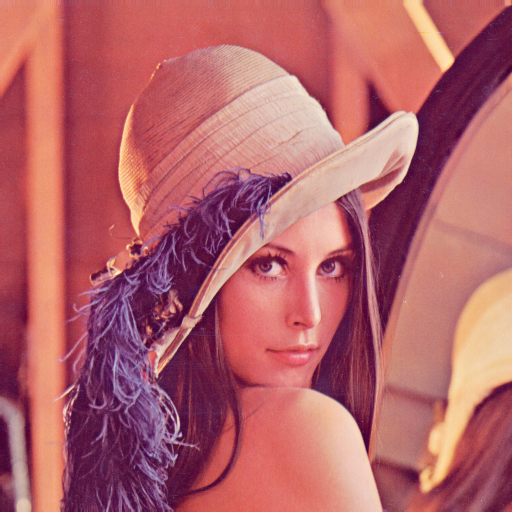
\includegraphics[width=0.40\textwidth]{../images/lena1.png}
	\caption{Immagine sorgente.}
	\label{fig:sorgente}
\end{figure}

\begin{figure}[ht]
\centering 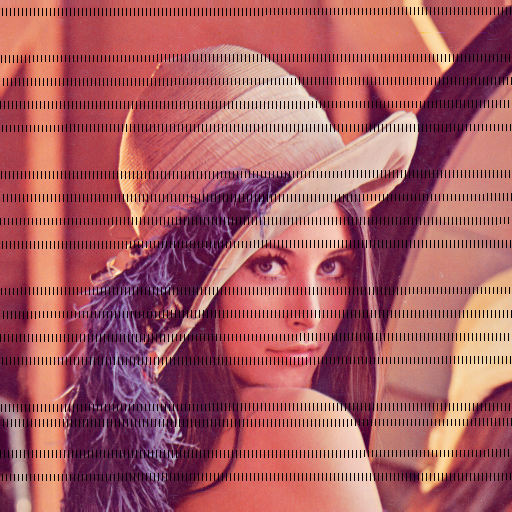
\includegraphics[width=0.40\textwidth]{../images/lena2.png}
	\caption{Immagine ricevuta.}
	\label{fig:ricevuta}
\end{figure}

\begin{figure}[ht]
\centering 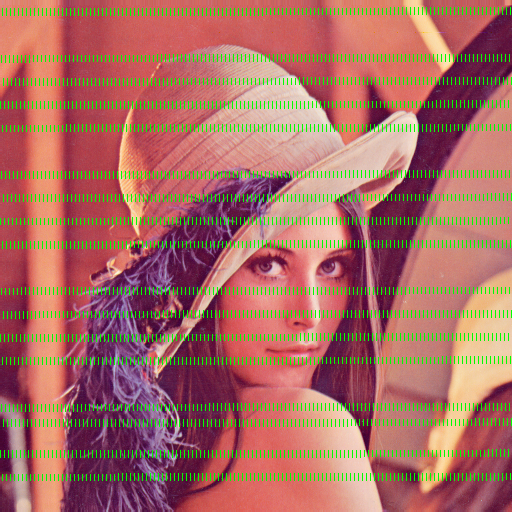
\includegraphics[width=0.65\textwidth]{../images/lena3.png}
	\caption{Evidenzioazione dei pixel non correttamente ricevuti.}
	\label{fig:evidenza}
\end{figure}

\begin{figure}[ht]
\centering 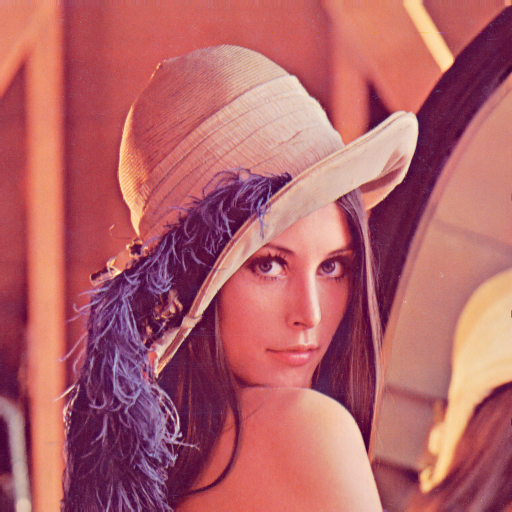
\includegraphics[width=0.65\textwidth]{../images/lena4.png}
	\caption{Immagine con i pixel mancanti interpolati.}
	\label{fig:interpolata}
\end{figure}

La figura \ref{fig:evidenza} mostra la totalità di pixel correttamente
ricevuti. In verde è possibile notare i pixel mancanti.
In figura \ref{fig:ricevuta} è mostrata l'immagine ricevuta.
Le immagini \ref{fig:sorgente}, \ref{fig:ricevuta}, \ref{fig:evidenza} e
\ref{fig:interpolata} permettono l'immediata visione del funzionamento del codec
nel suo complesso. Differentemente dal testo, l'immagine \ref{fig:sorgente} è stata codificata e inviata al destinatario, successivamente è stata decodificata. La
perdita di descrittori è casuale e dovuta alla congestione o
inefficienza della rete. Tutte le 4 descrizioni in cui è stata codificata
l'immagine sorgente sono state correttamente decodificate.
Si può notare che la figura \ref{fig:interpolata} presenta delle imperfezioni
dovute esclusivamente alla perdita dei pixel associati ai descrittori persi (17 su 195) durante il trasferimento. In tali zone
dell'immagine è stato eseguito l'algoritmo di interpolazione. 